\documentclass[a4paper, 11pt]{report}
\usepackage[utf8]{inputenc}
\usepackage{amsmath,tabto}
\usepackage{hyperref}
\usepackage{titlesec}
\usepackage{graphicx}
\graphicspath{ {images/} }

\usepackage{fullpage} % changes the margin
\usepackage{setspace}
\titleformat{\chapter}[display]
  {\normalfont\bfseries}{}{0pt}{\Large}
 \titlespacing*{\chapter}{0pt}{-50pt}{40pt}
\onehalfspacing
\date{}
\title{SOEN 6481 - System Software Requirements Specification
\newline Deliverable-1}

\author{
\normalsize  {Maria Ahmed}\\
\normalsize  {Adarsh Aravind}\\
\normalsize  {Sri Akhil Varma Alluri}\\
\normalsize  {Dheeraj Ashok Shobha}\\
\normalsize  {Charles Jebalitherson Augustin Moses}}
\begin{document}
\maketitle

\chapter{Problem (1) Description of TVM}
Ticket Vending Machine (will be referred as TVM in this document) is a self service automated ticket distribution system where tickets are printed and delivered to the users for transportation purpose. In this project, we analyse the TVM of metro operator in montreal called STM(Société de transport de Montréal). STM's TVM involves variety of actors such as Government, STM, Payment authority, customer, station master,.. which makes it an interesting domain to study. \\\\
TVM is a stationary computerized machine installed in all metro stations. Every station has at-least one TVM installed in it for public use. STM provides two options of legal tender for transit namely Printed ticket and OPUS Card. Printed ticket is a small piece of paper, that gives holder a certain right to travel from a source to the destination. Printed ticket usually includes short term travels such as 1 trip, 2 trips, 3 day pass, Weekend unlimited trip,.. Drawback of printed ticket is its limited validity (Eg. 1 trip ticket expires within 120 minutes after it is validated).  On the other hand, OPUS card is a rechargeable, dual interface smart card using the Calypso Standard, ideally used for long term travel plans namely, Monthly pass, 4-month pass. Group tickets cannot be purchased using OPUS card. The travel fare varies based on different age groups of the user.\\\\
TVM offers two ways of payment methods such as Cash(maximum of \$80) and Card(Debit, Credit).
STM protects the customer information by handling the payments through high level secured communication protocol. TVM has in-built security feature  to validate the card, here TVM initiates a request to connect with financial institution server and validates the given card against the PIN entered by the user. STM has a strong established network that handles thousands of users on a daily basis and it is highly reliable.\\\\
TVM is also used to assist in management of queue and priority of services in financial institutions, universities, and customer help desks of several organizations. It saves the time, money and effort by providing the services in a quick and efficient manner. TVM is highly available but fails rarely due to power outage, internet service breakdown and other TVM machine related problems.\\

\qquad\qquad\qquad\qquad 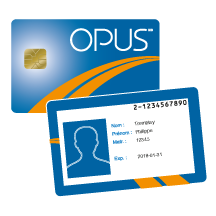
\includegraphics[width=70mm,scale=0.5]
{opus.png}\\
\tab\tab\qquad\qquad Fig.1 Sample of OPUS card (Source: Carte OPUS)
\end{document}
